% $Id: template.tex 11 2007-04-03 22:25:53Z jpeltier $

\documentclass{vgtc}                          % final (conference style)
%\documentclass[review]{vgtc}                 % review
%\documentclass[widereview]{vgtc}             % wide-spaced review
%\documentclass[preprint]{vgtc}               % preprint
%\documentclass[electronic]{vgtc}             % electronic version

%% Uncomment one of the lines above depending on where your paper is
%% in the conference process. ``review'' and ``widereview'' are for review
%% submission, ``preprint'' is for pre-publication, and the final version
%% doesn't use a specific qualifier. Further, ``electronic'' includes
%% hyperreferences for more convenient online viewing.

%% Please use one of the ``review'' options in combination with the
%% assigned online id (see below) ONLY if your paper uses a double blind
%% review process. Some conferences, like IEEE Vis and InfoVis, have NOT
%% in the past.

%% Figures should be in CMYK or Grey scale format, otherwise, colour 
%% shifting may occur during the printing process.

%% These three lines bring in essential packages: ``mathptmx'' for Type 1 
%% typefaces, ``graphicx'' for inclusion of EPS figures. and ``times''
%% for proper handling of the times font family.

\usepackage{mathptmx}
\usepackage{graphicx}
\usepackage{times}
\usepackage{url}

\usepackage[tight,normalsize,sf,SF]{subfigure}

\setlength\fboxsep{0pt}

\onlineid{174}

%% declare the category of your paper, only shown in review mode
\vgtccategory{Research}

%% allow for this line if you want the electronic option to work properly
\vgtcinsertpkg

%% Paper title.

\title{VCMass: A Framework for Verification of Coronal Mass Ejection Ensemble Simulations}

\author{
Alexander Bock\thanks{e-mail: \{ alexander.bock $\vert$ anders.ynnerman $\vert$ timo.ropinski \}@liu.se}
\and M. Leila Mays\thanks{e-mail: \{m.leila.mays $\vert$ lutz.rastaetter-1 \}@nasa.gov}
\and Lutz Rastaetter$^\dagger$
\and Anders Ynnerman$^*$
\and Timo Ropinski$^*$\\
\and
\scriptsize $^*$ Department of Science and Technology, Link\"oping University, Sweden\\%
\scriptsize $^\dagger$ NASA Goddard Space Flight Center, Greenbelt, MD, USA
}
%\author{
%    Alexander Bock
%\and
%    M. Leila Mays
%\and
%    Lutz Rastaetter
%\and
%    Anders Ynnerman
%\and
%    Timo Ropinski
%    
%%    \scriptsize Link\"oping University\\%
%%    \scriptsize Goddard Space Flight Center, NASA
%
%}

%\author{%
%    Alexander Bock\thanks{e-mail: alexander.bock@liu.se}\\%
%    \scriptsize Link\"oping University%
%\and
%    M. Leila Mays\thanks{e-mail: m.leila.mays@nasa.gov}\\%
%    \scriptsize Goddard Space Flight Center, NASA\\
%\and
%    Lutz Rastaetter\thanks{e-mail: lutz.rastaetter-1@nasa.gov}\\%
%    \scriptsize Goddard Space Flight Center, NASA
%\and
%    Anders Ynnerman\thanks{e-mail: anders.ynnerman@liu.se}\\%
%    \scriptsize Link\"oping University%
%\and
%    Timo Ropinski\thanks{e-mail: timo.ropinski@liu.se}\\%
%    \scriptsize Link\"oping University%
%}

\abstract{%
Supporting the growing field of space weather forecasting, we propose a framework to analyze ensemble simulations of coronal mass ejections. As the current simulation technique requires manual input, uncertainty is introduced into the simulation pipeline which leads to inaccurate predictions. Using our system, the analyst can compare ensemble members against ground truth data (arrival time and geo-effectivity) as well as information derived from satellite imagery. The simulations can be compared on a global basis, based on time-resolved quality measures, and as a 3D volumetric rendering with embedded satellite imagery in a multi-view setup. This flexible framework provides the expert with the tools to increase the knowledge about the, as of yet not fully understood, principles behind the formation of coronal mass ejections.

%By extracting the optical flow from the images and renderings, we retrieve pairs of velocity fields that are utilized to derive a quality measure that is used to test the simulation against the ground truth satellite image data. The system provides techniques to simultaneously inspect the time-dependent quality measures of all observation instruments (SOHO [LASCO C3], STEREO A and B [Cor2, HI 1, and HI 2]) and allow the analyst to make an informed decision about the accuracy of the simulation.


%The current technique of simulating coronal mass ejections in ENLIL simulations requires cone parameters that are manually derived from STEREO satellite imagery. This manual input is not perfect and introduces uncertainty into the simulation pipeline, leading to inaccurate predictions. We present a system that embeds satellite imagery from SOHO and STEREO A and B into a 3D volumetric rendering of ENLIL simulations. By extracting the optical flow from the images and renderings, we retrieve pairs of velocity fields that are utilized to derive a quality measure that is used to test the simulation against the ground truth satellite image data. The system provides a novel technique to simultaneously inspect the time-dependent quality measures of all observation instruments (SOHO [LASCO C3], STEREO A and B [Cor2, HI 1, and HI 2]) and allow the analyst to make an informed decision about the accuracy of the simulation. Lastly, we extend this system to deal with ensemble runs, generated by varying the cone parameters. The aforementioned quality measures are generated for each ensemble member and the system provides an interface to browser and assess the whole ensemble run at once, enabling the analyst to quickly select the ensemble member agreeing with the satellite data.

}

\def\etal{\textit{et al.}}


%%%%%%%%%%%%%%%%%%%%%%%%%%%%%%%%%%%%%%%%%%%%%%%%%%%%%%%%%%%%%%%%
%%%%%%%%%%%%%%%%%%%%%% START OF THE PAPER %%%%%%%%%%%%%%%%%%%%%%
%%%%%%%%%%%%%%%%%%%%%%%%%%%%%%%%%%%%%%%%%%%%%%%%%%%%%%%%%%%%%%%%%

\begin{document}

\firstsection{Introduction}
\maketitle

\emph{Space weather} is the description of the environmental conditions in our solar system and the effects it has on planets and spacecraft. Coronal mass ejections (CMEs) occur when the magnetic field lines on the Sun reconnect, providing massive amounts of acceleration to a plasma cloud and ejecting it into the solar system. \emph{Space weather forecasting} is amongst others the endeavour of predicting the direction, velocity, and impact factor of CMEs when they hit objects in the solar system, like Earth or man-made spacecraft. The biggest event on record is the Carrington Event from 1859 that generated auroras as far south as the Sahara and damaged telegraph lines worldwide. It is estimated that in North America alone a similar event today would cause up to \$2.6 trillion in damages and blackouts of up to 2 years due to destroyed transformers, a situation that can be almost completely mitigated by accurate forecasting \cite{lloyds2013impact}.

Current predictions are based on simulations, whose input parameters are derived from satellite imagery. In our system, we are using the widely used magnetohydrodynamic (MHD) simulation code ENLIL~\cite{odstrcil2003modeling} with the Wang-Sheeley-Arge model~\cite{parsons2011wang}, where the CME is modelled as a cone with position, velocity, and opening angle as free parameters. The cone parameters are then used to generate initial condition for the MHD simulation. Currently, parameters are manually derived from satellite images, which naturally introduces error into the simulation and thus requires verification. While the ENLIL-WSA simulation is the current state-of-the-art approach, the assumption of a conical shape of the CME is not true in general, further increasing the need for a flexible verification tool.

To weaken the impact of measurement errors, simulation ensembles are generated by varying the free parameters and performing the simulation for each combination. A simulation run can be verified in two ways. One, if the CME impacts the Earth or any suitable spacecraft in the solar system, ground-truth in-situ measurements of the arrival time, velocity, and strength are recorded and are compared against the predicted values. Second, the time-evolution of the CME in the simulation can be visually compared to recordings from spacecraft equipped with coronagraph imagers. Currently, there are three active spacecraft capable of this; the SOHO is located at the L$_1$ point between Earth and the Sun and STEREO A and STEREO B are on heliocentric orbits. STEREO A and B have three separate imagers ranging from the Sun's surface all the way to the orbit of the Earth.

Our proposed system provides the space weather analyst with the visualizations to quickly assess the quality and accuracy of each ensemble member, the possibility to inspect the time-dependent error broken down by each available satellite and instrument, and finally to inspect a 3D rendering of the simulation results integrated with the positions of different spacecraft, their instrument fields, and planetary bodies.

\section{Related Work}
Notable work dealing with the visualization of ensembles was done by Bruckner and M\"oller, who developed a system to explore a simulation parameter space allowing a user to reach a desired result~\cite{bruckner2010result}. The main difference to our framework is the unknown desired result. Naturally, many similarities are present with the field of weather forecasting on Earth, which has greatly matured over the years. Sanyal \etal\ developed a system to explore ensemble simulations for weather forecasting that is most similar to ours~\cite{sanyal2010noodles}. However, due to the inherent differences in weather forecasting compared to space weather forecasting (2.5D structures vs full 3D structures, the limited amount of measurement points, and theoretical frameworks that are missing), their approach is not applicable to space weather.

The validity of time-dependent comparisons of CME simulations with satellite data was shown in related work by Manchester \etal ~\cite{manchester2008three} and Rusin \etal ~\cite{rusin2010comparing}, while Lugaz analyzed the expected accuracy and possible sources of error in this method~\cite{lugaz2010accuracy}.

\section{Framework Overview}
\begin{figure}
\subfigure[Ensemble Selection View]{
    \fbox{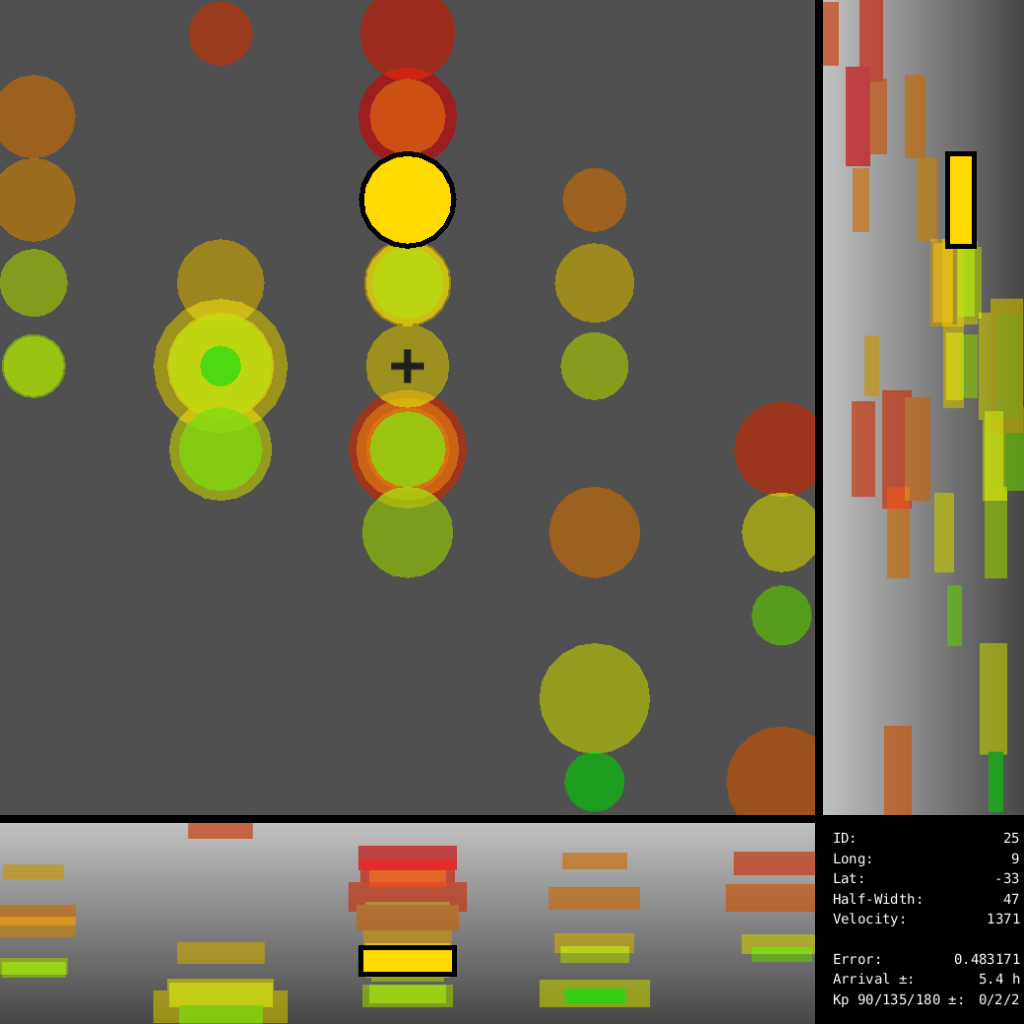
\includegraphics[width=0.49\linewidth]{figures/selection.png}}
    \label{fig:selection}
}
\subfigure[Rendering View]{
    \fbox{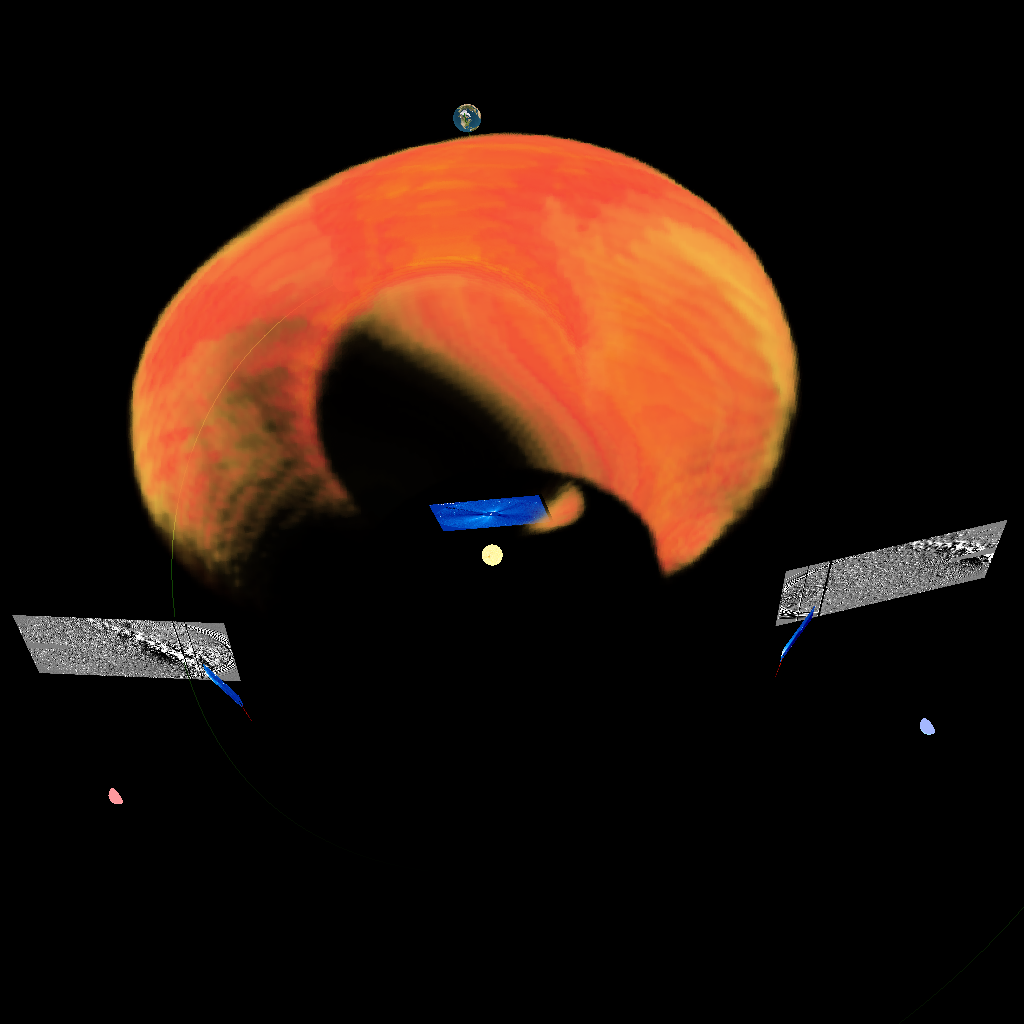
\includegraphics[width=0.49\linewidth]{figures/rendering.png}}
    \label{fig:rendering}
}
\\
\subfigure[Timeline View]{
    \fbox{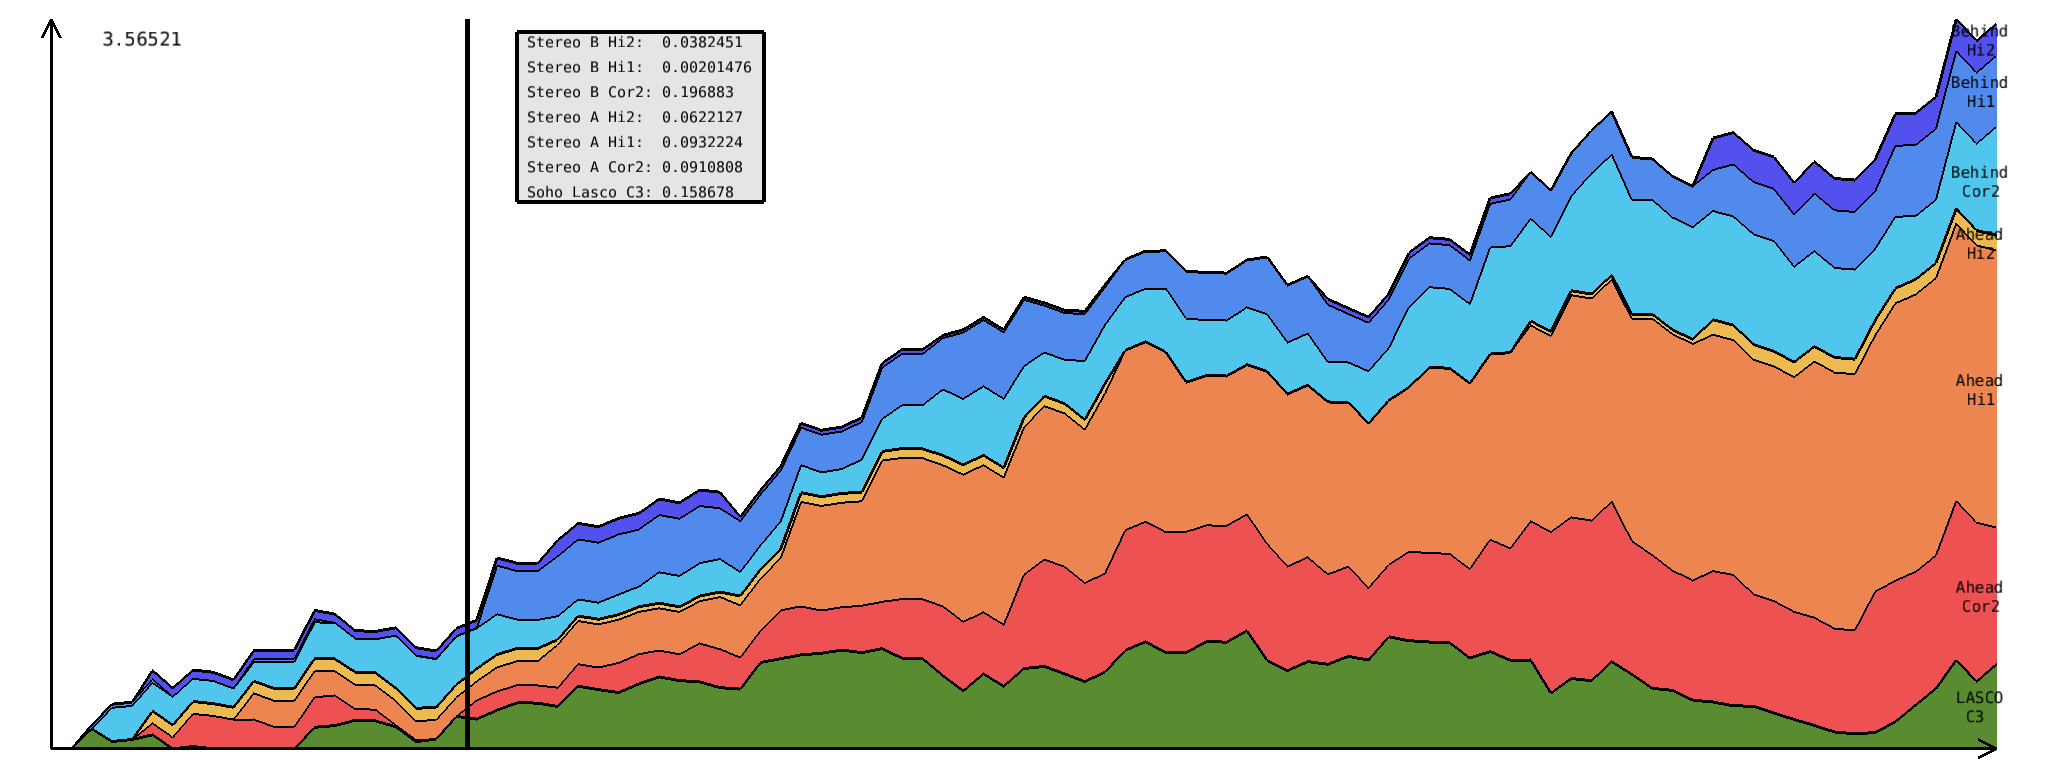
\includegraphics[width=\linewidth]{figures/river.png}}
    \label{fig:timeline}
}
\caption{The three different views in our framework providing the space weather analyst tiered access to the data necessary to compare ensemble members. Please note that the sizes of planetary bodies in (b) are exaggerated by 750$\times$ and the Sun by 5$\times$.}
\label{fig:system}
\end{figure}

Figure~\ref{fig:system} shows our multi-view framework applied to an event that occurred on April 18th, 2014. In this section, we describe available data (Section~\ref{sec:data}), the \emph{Ensemble Selection View} (Section~\ref{sec:selection}), the \emph{Timeline View} (Section~\ref{sec:timeline}), and the \emph{Rendering View} (Section~\ref{sec:rendering}). The workflow for the analyst is to inspect the Ensemble Selection View first, getting an overview of the accuracy and validity of ensemble members. Afterwards, the Timeline View is utilized for a subset of interesting ensemble members to gain a deeper understanding of the time-dependent comparisons, grouped by satellites and instruments. Finally, the Rendering View is used to inspect the specific time steps that were used for the comparison by viewing the volumetric rendering of the CME embedded with the satellite images, spacecraft, and planetary bodies.

\subsection{Data} \label{sec:data}
In our test case, the following data was available. The ENLIL ensemble run consists of 36 members, each providing a 4D volume with a cadence of about 1 hour with the data stored on a spherical grid. Each voxel contains the particle count, plasma density, magnetic field direction, velocity, temperature, dynamic pressure, and others. The ground-truth data at Earth, i.e. arrival time, velocity, and magnetic field polarity of CMEs, comes from the ACE spacecraft orbiting the L$_1$ point. The geo-effectivity, the Kp-Index, is measured at different observation stations on Earth and determines how much the Earth's magnetic field is disturbed. Coronagraph images from three satellites are used; SOHO's Lasco C3 is a white-light coronagraph covering 3.7 to 32 solar radii. From the identical STEREO A and B spacecraft, we utilize one coronagraph imager (COR2), covering 2.5 to 15 solar radii, and the two heliospheric imagers (HI1 and HI2), covering 15-90 solar radii and 70-330 solar radii respectively. Using these images, a continuous monitoring of a CME from the Sun's surface towards Earth is possible.

\subsection{Ensemble Selection View} \label{sec:selection}
The Ensemble Selection View (Figure~\ref{fig:selection}) provides an overview of the ensemble members and their validity. Each ensemble member is characterized by 3 parameters: location (longitude and latitude), initial velocity, and the cone's opening angle. In all three subviews, the opening angle is mapped to the size of the glyph. The main view (top left) shows the longitude and latitude on the horizontal and vertical axes, the side views show longitude vs. velocity (bottom left) and latitude vs. velocity (top right). The color mapping can be changed between imaged-based comparison, arrival time, and Kp index, allowing detailed inspection of the two ground truth and the derived accuracy measure. Ensemble members are selected by the user, which highlights the glyph and provides additional information in the lower right corner. 

\subsection{Timeline View} \label{sec:timeline}
When an ensemble member is selected in the Ensemble Selection View, its timeline is presented (Figure~\ref{fig:timeline}). This view shows the time-dependent error for each of the instruments for each satellite. The information is grouped into three parts. First, the combined error for all satellites and instruments is presented. Second, the error is broken down for each satellite and shown as a stacked graph providing access to the individual error. Third, in the most detailed view the individual errors for the instruments are shown enabling detailed analysis of the potential sources of error in the simulation. For each mode a highlight follows the mouse and provides detailed information for each instrument at the selected time step. A stacked graph was chosen as it was shown that they are better suited for reading the overall trend~\cite{byron2008stacked}, a characteristic that was important for the overall error. The colors of the stacks have been selected to maintain a mental linking between instruments and their satellites. A primary color was chosen for each satellite, and perceptually similar colors are used for the corresponding instruments.

The algorithm used for computing the time-varying error is deliberately held flexible. Currently, we are experimenting with an approach that uses optical flow analysis~\cite{sun2010secrets} and a perceptual difference metric~\cite{yee2004perceptual} to compare a rendering of the simulation data with the satellite imagery.

\subsection{Rendering View} \label{sec:rendering}
Selecting a time step in the Timeline View will set up the scene in the 3D rendering to provide a detailed view (Figure~\ref{fig:rendering}). The ENLIL volume data is loaded, the spacecraft and planets are at their correct positions, and the satellite images for each instrument are loaded and shown in place using perspective texturing. The volumes are stored in a spherical coordinate system, meaning that the 3D texture stores $r$, $\phi$, and $\theta$ in the principal axes. Raycasting is performed in the Cartesian world space with each sample point along a ray converted into a spherical coordinate that is then used for lookup. This allows both for an adaptive sampling scheme, as there is more data available closer to the origin, as well as an more accurate interpolation scheme based on SLERP interpolation.

\bibliographystyle{abbrv}
\bibliography{bibliography}
\end{document}
